\chapter{Theme 4: in-silico Pre-clinical Trials for Implantable Cardiac Devices} 
\section{Clinical trials and RIGHT}
\label{sec:rcts}

At the clinical trial stage (Fig.~\ref{fig:spectrum}), the objective is no longer to find bugs in the device: it is, rather, to evaluate the safety and efficacy of the validated device on humans. 
RCT are the gold standard for evaluating the safety and efficacy of a new medical device \cite{FriedmanFD10_ClinicalTrials}.
They constitute the only time prior to market use where the effects of the device on humans are actually observed, and are legally mandated for new high-risk medical devices like ICD.
%It is important to understand how a typical RCT proceeds to appreciate where CPS modeling can help in that process.
%Very broadly, in an \ac{RCT}, a new treatment also known as the \emph{intervention}, is compared to the current standard of care, commonly known as the \emph{control}.
%For example, two competing ICDs are compared.
%Each patient recruited to the trial is randomly assigned to either the intervention or the control group and undergoes the corresponding treatment.
%At the end of the trial, any clinically relevant differences between the two groups are evaluated to determine if they are statistically significant.
The planning and execution of an RCT requires carefully navigating a number of technical, logistical and ethical issues to obtain reliable and statistically significant results.

Because of the very high cost of RCT in terms of money, time, and the risk of harm they present to enrolled patients, our focus in this paper is on the use of CPS models, formalized in an MBCT, \emph{to validate the assumptions made by the investigators and thus increase the chances of success of an RCT}.
We illustrate our approach by applying it to the Rhythm ID Going Head-to-Head Trial (RIGHT) \cite{GoldABBTB11_RIGHTresults}, which we present next.

\subsection{The RIGHT trial}
\label{sec:right}
We first provide a brief background to better understand RIGHT (see Fig.\ref{fig:icd}). Tachycardias (abnormally elevated heart rates) can be divided into VT, which originate in the heart's ventricles, 
and SVT, which originate above the ventricles.
A sustained VT can be fatal, while an SVT is typically non-fatal.
The therapy applied by the ICD often takes the form of a high-energy electric shock.
The shock can be pro-arrhythmic, and was even linked to increased morbidity \cite{shock_mortality}.
Therefore, one of the biggest challenges for ICDs is to guarantee shock delivery for VT, and simultaneously reduce inappropriate shocks during SVT \cite{Ellenbogen11_Pacingbook}.

RIGHT is a trial that sought to compare the VT/SVT discrimination abilities of two algorithms \cite{GoldABBTB11_RIGHTresults}: 
the Rhythm ID detection algorithm found in Boston Scientific's Vitality II ICDs~\cite{compass},
and the PR Logic + Wavelet (PRL+W) detection algorithm found in a number of Medtronic's ICDs (Medtronic Maximo,
Marquis, Intrinsic, Virtuoso, or Entrust ICD).
%\mynote{SD}{make sure to list all the Boston Scientific and Medtronics ICD models that use each of these algorithims. This is very important}
%The investigators chose the following primary question: is there a difference in time-to-first inappropriate therapy between the two ICDs?
\emph{Inappropriate therapy} was defined as therapy applied to an arrhythmia other than VT or VF (VF is a type of VT).
RIGHT enrolled 1962 patients and ran for approximately five years.
It was fully sponsored by Boston Scientific. 

One of the trial's assumptions was that Rhythm ID would reduce the risk of inappropriate therapy by 25\% over PRL+W~\cite{Berger06_RIGHT}.
The outcome of the trial~\cite{GoldABBTB11_RIGHTresults}, however, was that patients implanted with ICDs running Rhythm ID had a \emph{\textbf{34\% risk increase}} of inappropriate therapy as compared to patients implanted with ICD running PRL+W. 
This result  is the opposite of the effect hypothesized by the trial investigators. 
In this paper, we design an MBCT to test early and quickly whether the hypothesized effect holds by comparing the two ICDs on a large \emph{synthetic} cohort.\\\\
\textbf{\emph{Organization:}} In the following sections we describe the building blocks of the MBCT: modeling the heart, processing 100's of real patients' data, mapping the timing and morphology components of the signal to a heart model we developed, generating a population of 10,000+ synthetic heart models, implementing the device algorithms and conducting multiple trials for the comparative rate of inappropriate therapy, condition-level rates and evaluating the effect of device parameters on discrimination rates.

 \section{Heart Modeling}
 \label{sec:heart modeling}
%The first step in any MBCT is to choose a patient model that can interact with the device in a closed loop. 
%Computer models of the heart have been developed to model different aspects of the cardiac function to suit different applications (\cite{natalia,Grosu_wave}).
%In this section we first give a brief overview of the basic Electrophysiology of the heart which describes the electrical activation and conduction, which is the basis for ICDs. 
%We also describe our effort to model the electrical activity of the heart to generate signals corresponding to a large range of heart conditions that the ICD can encounter.

\subsection{Basic cardiac electrophysiology}
\label{sec:cardiac ep}
The heart has two upper chambers called the \emph{atria} and two lower chambers called the \emph{ventricles} (see Fig. \ref{fig:icd})
The synchronized contractions of atria and ventricles assure an adequate supply of oxygenated blood to the rest of the body.
This contraction is driven by electrical activity in the heart.
A normal pattern of electrical activity is referred to as NSR.
Disturbances of NSR are referred to as \emph{arrhythmias}, and can result in insufficient blood supply and even death of a patient. 
\emph{VT} is an example of an arrhythmia originating in the ventricles, in which the ventricles beat at a very high rate.
If the VT is sustained, or degenerates into VF, it is fatal within seconds.
An abnormally fast heart rate that originates in the atria and/or the conductinon system above the ventricles is referred to as a \emph{SVT}.
This is not a fatal condition but does cause patient discomfort and its treatment is elective.
Many arrhythmias fall under this heading.

Implantable Cardioverter Defibrillators (ICDs) can diagnose VT and VF by observing the electrical activity through three channels, as shown in Fig.~\ref{fig:icd}.
The measured signals are known as \emph{electrograms}, or EGMs.
VT and SVT can share similar heart rates and might even occur simultaneously, so an SVT can be mis-diagnosed as a VT. 
This is problematic because VT therapy consists of low and high energy electric shocks of 30-40 Joules ($\sim$800V) delivered directly to the heart, which is very painful to the patient, and has been shown to increase morbidity \cite{shock_mortality}\footnote{\small{Physicians compare a shock to a ``horse kicking you in the chest"}}.
Therefore, one of the biggest challenges for ICDs is to discriminate between VT that typically requires a shock, and SVT that typically should not be shocked \cite{Ellenbogen11_Pacingbook}.

An EGM signal can be characterized by the \emph{timing of events} that produced it, and the \emph{morphology of the signal itself}.
An `event' is roughly characterized as the source of the largest peak in the EGM (e.g. a ventricular depolarization), and event timing is a crucial element of an arrhythmia's definition in clinical Electrophysiology.
The `morphology' refers to the shape of the EGM (see Fig. \ref{fig:adjudication} for examples).
Both aspects are used by the ICD to make its decision.
Correspondingly, our model has two components: a timing model, and a morphology model.

\subsection{Timing Model}
\begin{figure}[t]
	\centering
	\vspace{-10pt}
	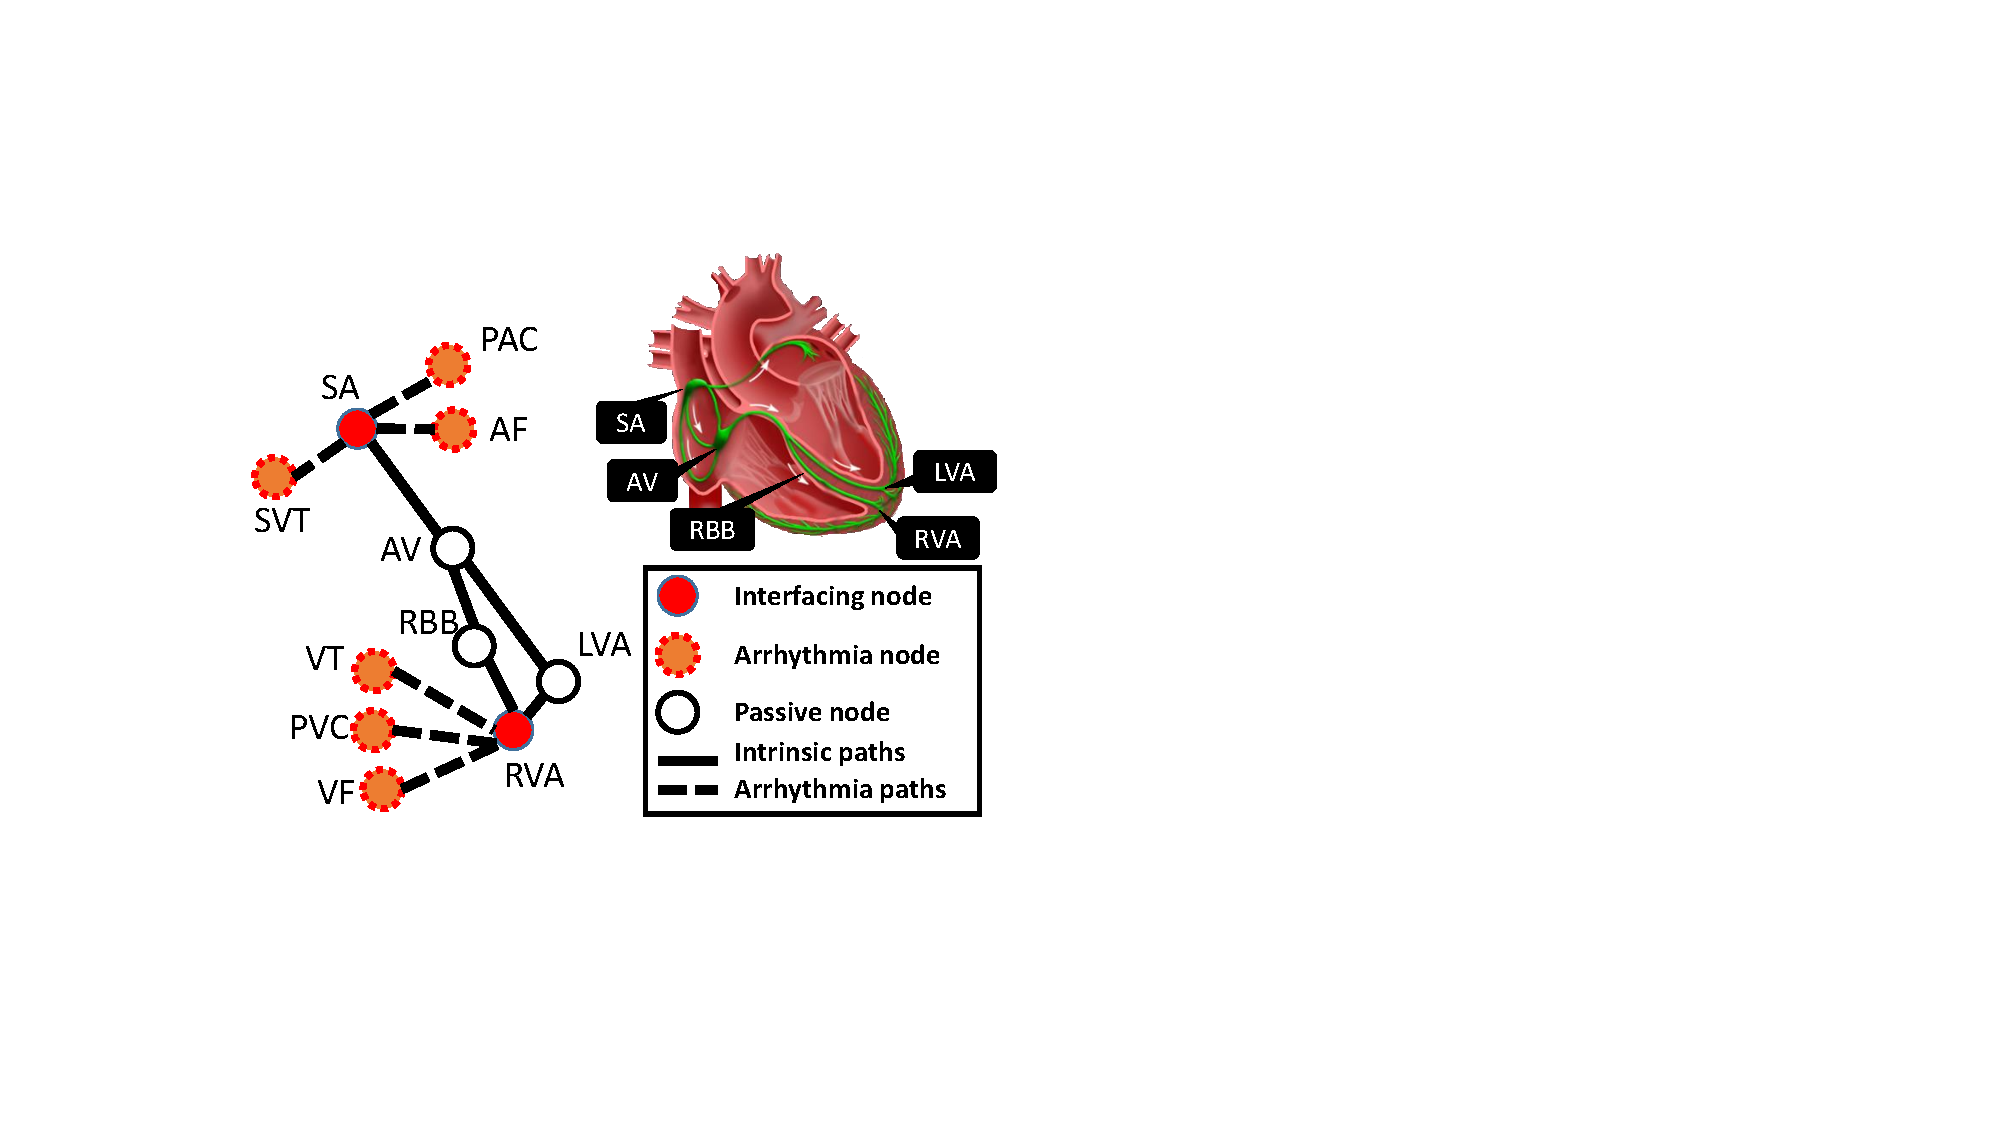
\includegraphics[width=0.3\textwidth]{figs/HM_top.pdf}
	\caption{\small Timing model of the heart}
	\vspace{-10pt}
	\label{fig:HM_top}
\end{figure}
Computer models of the heart have been developed to model different aspects of the cardiac function to suit different applications (\cite{natalia}).
In \cite{VHM_proc}, the authors developed a heart model structure that can be used to simulate the timing for generation and conduction of electrical events of the heart under a variety of conditions.
The model structure consists of a set of node automata, which model the \emph{generation} and \emph{blocking} of electrical events by heart tissue, and a set of path automata, which model the \emph{conduction delay} of electrical activity between node automata.
The node and path topology used in the MBCT is shown in Fig. \ref{fig:HM_top}. 
The hollow nodes are passive nodes representing key locations within the heart where electrical events may be blocked. These include the Atrioventricular node (AV), Right Bundle Branch (RBB) and Left Ventricle Apex (LVA). 
The filled nodes in red, Sinoatrial (SA) node and Right Ventricle Apex (RVA) node, represent the heart locations where ICD electrodes are placed to measure the EGMs.
The timing of the activation events at these nodes determines the timing of corresponding EGMs.
Different sources for tachyarrhythmias are represented by arrhythmia nodes (dashed filled nodes) which are capable of self-activating at prescribed rates. These include Premature Atrial Complexes (PACs) and Premature Ventricular Complexes (PVCs) which are sources of rhythm disturbances.

Every node and path automaton has timing parameters that determine, for example, the delay between events, and how long it takes to conduct an electrical event between two nodes.
These timing parameters can be directly derived from clinical data \cite{josephson}, and the model structure is compatible with clinical Electrophysiology concepts.
Thus we know the ranges for these parameters.
In \cite{VHM_proc}, the timing model's capability to simulate various normal and abnormal heart conditions was validated quantitatively and by cardiac electrophysiologists.


In this work we use the same heart model structure to ensure the correct timing of the EGM signals into the ICD.
%The nodes in orange are capable of self-activation at different rate determined by corresponding parameters, which represent different sources for tachy-arrhythmia.
%Since in this study we do not need the heart models to react to device therapy.
In order to account for inherent timing variability, during simulation the heart model randomly selects timing parameters within a pre-specified range, instead of choosing specific values. 
By choosing the range, we control the variability of the signals produced by a given model instance.

\subsection{Morphology Model}
The ICD uses the EGM morphology in two ways:
first, the atrial and ventricular EGMs are used to \emph{sense} when events occur via peak detection (Section \ref{sec:sensing}).
Second, the Shock channel EGM is used in the morphology comparison discriminators (Section \ref{sec:svtvt}, \cite{VTC,Wavelet}).
It is known that sensing (the detection of events) can be responsible for up to 20\% of inappropriate therapies \cite{wrong_sensing}.
Therefore, it is important that our model generate realistic and varied EGM waveforms for a proper evaluation of the detection algorithms.

\begin{figure}[t]
	\centering
%	\vspace{-5pt}
	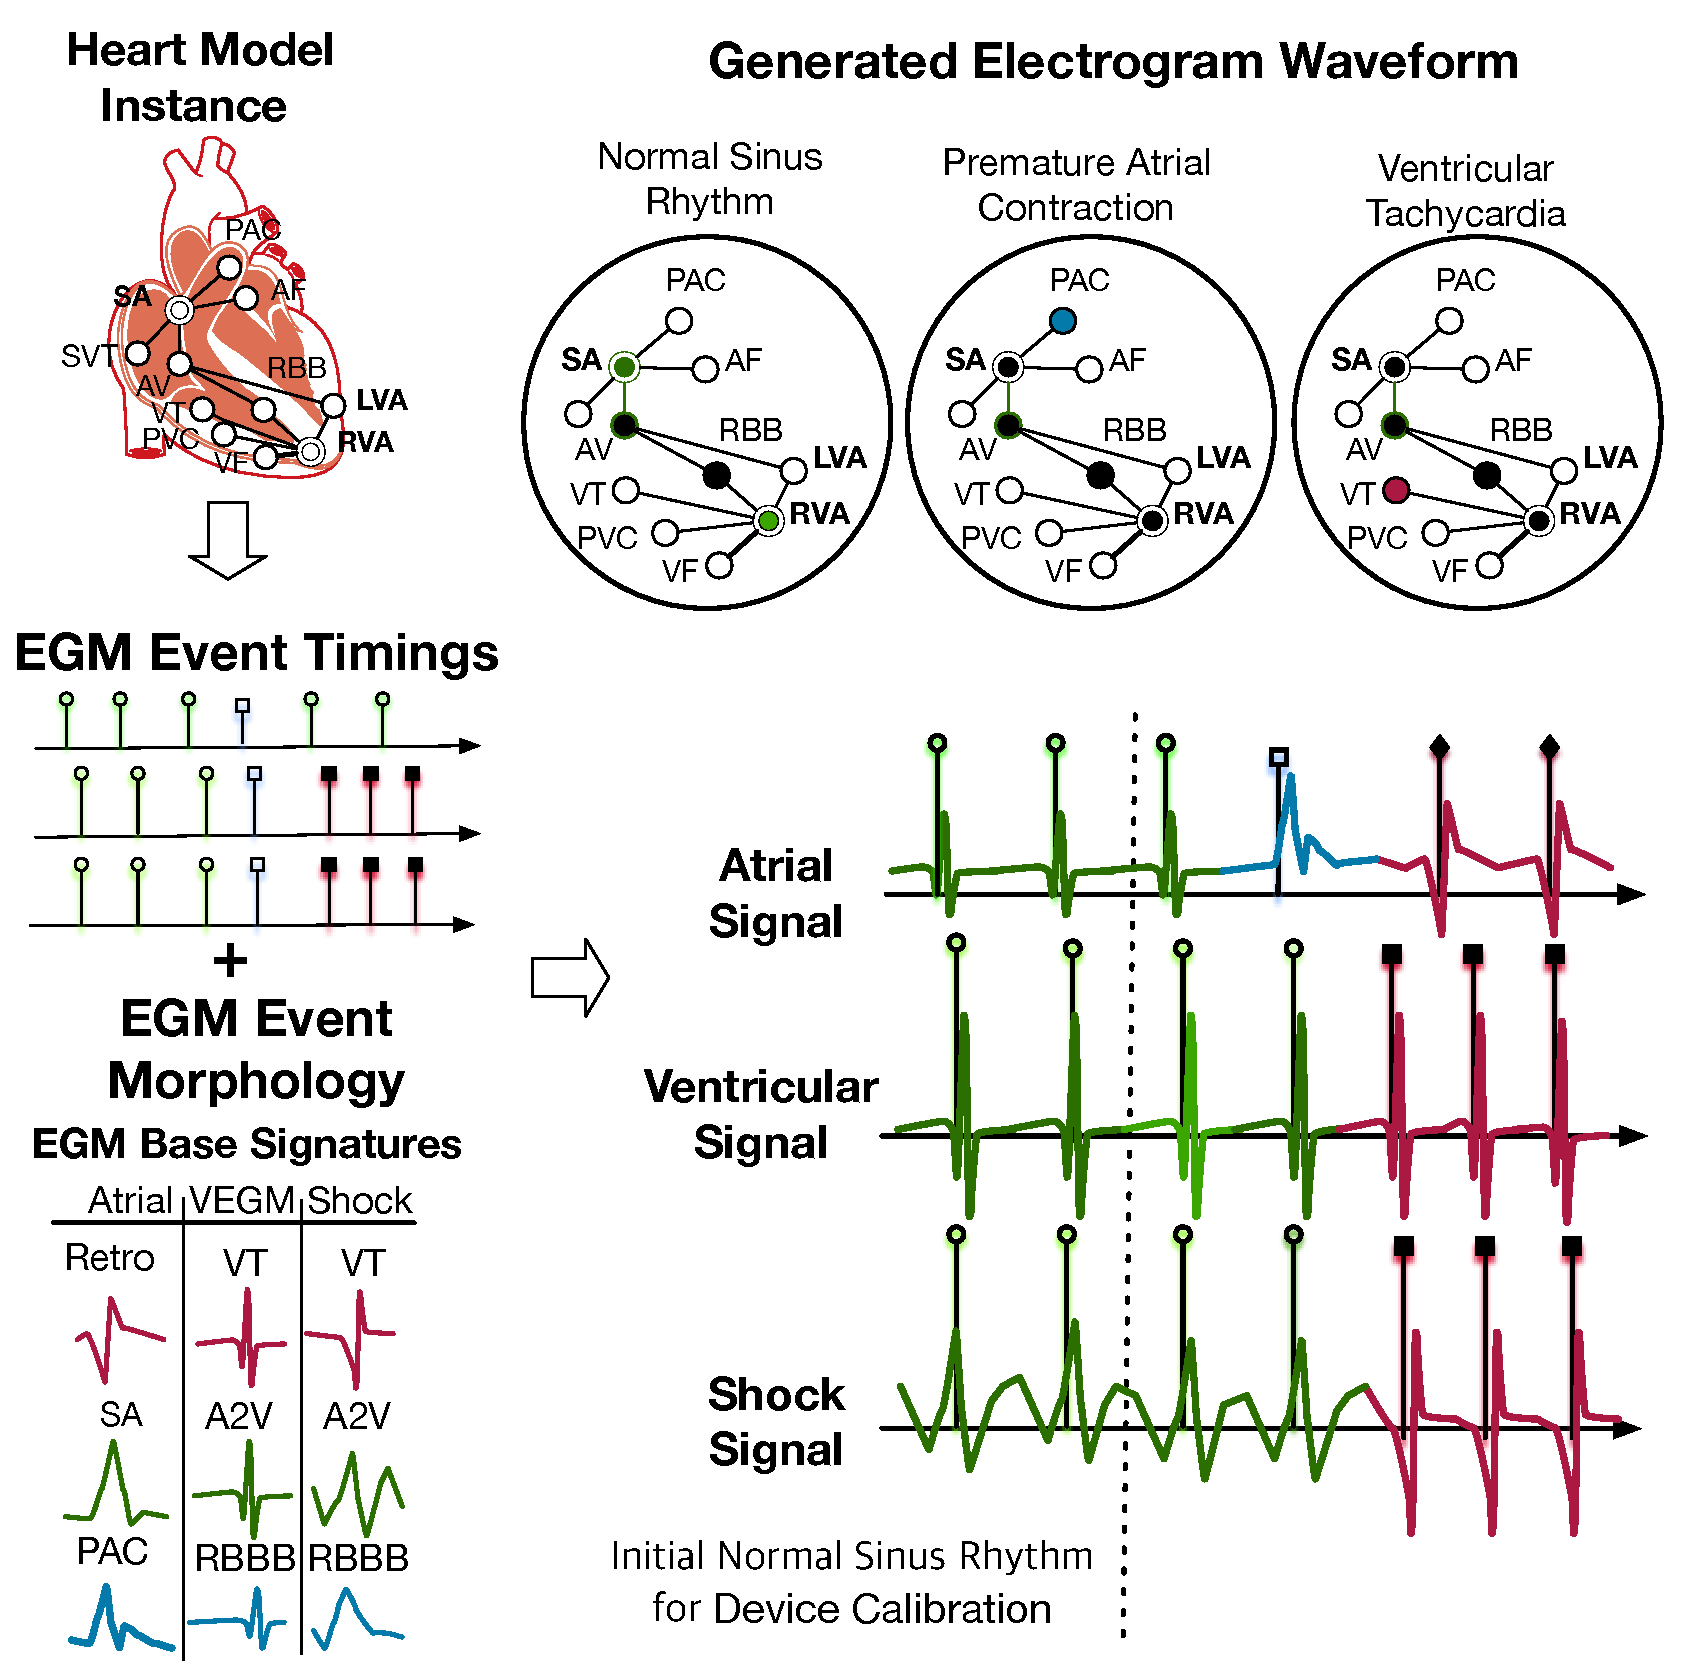
\includegraphics[scale=0.3]{figures/figEGMGeneration1column.pdf}
	\vspace{-15pt}
	\caption{\small EGM waveform generation.
		From a given model instance and set of tachycardias, an EGM waveform is generated for the duration of an episode. The timing model determines event timings. When an event occurs, the EGM morphology for the event is output from the morphology model.  
		}
	\vspace{-15pt}
	\label{fig:egmGeneration}
\end{figure}
The timing model provides the time stamps for electrical events to happen at the interfacing nodes (SA,RVA). 
From path conduction we also know the source of the signals.
In the heart model structure shown in Fig. \ref{fig:HM_top} there are 5 different sources for SA node activation and 5 different sources for RVA node activation. 
Based on the clinical observations that electrical events from the same source produce very similar EGM morphologies, we can generate EGM signals by overlaying EGM templates corresponding to different sources onto the timing event diagram.
The procedure is shown in Fig. \ref{fig:egmGeneration}.
We also introduce small variations on EGM templates.
The variations are obtained by a wavelet decomposition of the signatures followed by a random scaling of the 25\% smallest coefficients.
We guarantee that this does not change the signature of the EGM, by running one of the morphology comparison discriminators described in Section \ref{sec:svtvt}.
This variation is parametrized, e.g. the percentage of modified coefficients, the range of the random scaling.

\subsection{Patient Data Adjudication and EGM Template Extraction}
In order to obtain realistic morphologies for our simulations we utilize the Ann Arbor Electrogram Libraries (AAEL), a database of over 500 EGM recordings made during clinical electrophysiology studies~\cite{AAEL}. 
The AAEL is used by all major ICD manufacturers and is licensed by the US FDA. 
The AAEL provides descriptive annotations of records at a high level.
We performed additional detailed examination to precisely segment each record according to rhythm type.
123 records from 47 patients were manually examined and adjudicated into segments called \emph{episodes} containing one specific rhythm, e.g. NSR or VF. 
The adjudication was performed by a cardiologist.
Fig. \ref{fig:adjudication} (left) shows an example record (Record A185660) which has undergone this adjudication.
%It should be noted that only with a standard 12-lead \ac{ECG} in addition to ICD signals can all types of arrhythmia be accurately diagnosed.
From each episode, we developed an automated process which extracted EGMs from a given episode. 
The EGM are collected and organized by both patient record and by the type of rhythm which was annotated during the adjudication process.
These extracted rhythm \emph{signatures} provide the basis for the morphology information in the signal generated by our model.
Fig. \ref{fig:adjudication} (right) depicts an example of 10 signatures extracted from the record. 

\begin{figure*}[t]
	\centering
	\vspace{-10pt}
	\includegraphics[scale=0.35]{figures/figadjudication.pdf}
	\vspace{-10pt}
	\caption{\small  (Left) The EGM record is segmented into episodes with distinct rhythms in each. (Right) From each episode, individual EGM morphologies are extracted and stored.
	}
	\label{fig:adjudication}
\end{figure*}

\subsection{Cohort generation}
\label{sec:cohort generation}
Let $p = (p_1,\ldots,p_n) \in \Re^n$ be the vector of timing and morphological parameters of the heart model.
Let $P_i \subset \Re$ be the range of parameter $p_i$.
We generate a \emph{synthetic cohort} of $N$ probabilistic model instances.
To produce one of these instances, for each scalar parameter $p_i$, we randomly select a sub-interval $I_i$ of its range: $I_i \subset P_i$.
The sub-interval $I_i$ is chosen so that it fits with the tachycardia that this model instance is meant to simulate.
E.g., for modeling VT, the rest period of the VT node might be assigned the sub-interval $I_i = [260, 280]ms$, reflecting the firing rate in the ventricles.
%Two different instances of the same tachycardia will, in general, have different sub-intervals within $P_i$.
When a model instance is simulated, each parameter $p_i$'s value changes beat to beat by sampling it uniformly within its sub-interval $I_i$.
Thus each generated model is probabilistic to reflect inherent rhythm variability.

\section{Implementing Device Algorithms} 
\label{sec:device models}
Due to the limited sensing capability of ICDs, device manufacturers have developed different algorithms to identify the electrical events and correctly diagnose the cardiac arrhythmia as being VT or SVT.
In this paper we implemented the detection algorithm Rhythm ID of Boston Scientific \cite{compass,Ellenbogen11_Pacingbook},% [???Compass, pacingdefibrillation,VTC paper, ICD book, Ellenbogen].
and PRLogic+Wavelet (PRL+W) of Medtronic \cite{Singer,Wavelet}.
%In available literature on the evaluations of device algorithms descriptions of the device algorithms are not detailed enough for full implementation.
%To obtain the detailed implementation we further reviewed clinical execution traces from literature like \cite{Singer} to infer detailed executions of the algorithms. 
We also set up a testing platform to validate our implementations against real ICDs using conformance testing.
\subsection{Cardiac Signal Sensing}
\label{sec:sensing}

%Basic definition and principle
\emph{Sensing} is the process by which cardiac signals measured through the leads of the ICD is converted to cardiac timing events.
Appropriate sensing is essential for proper ICD detection algorithm operation which relies heavily on accurate event timing and morphology information provided by sensing. 
An \emph{event} corresponds to a depolarization in the heart and manifests as a displacement from the baseline amplitude of the signal.
In its simplest form, the sensing algorithm declares an event whenever the amplitude of the signal exceeds a given threshold.
Once an event has been declared, the peak of the amplitude is measured and a \emph{refractory period} begins, during which a consecutive event is ignored for a short period of time. 
This is to ensure that the same event is not counted repeatedly.

%Difficulty of sensing
ICDs require a balance in sensitivity in order to operate in noisy, complex, environments where cardiac events can vary greatly in signal amplitude and frequency, such as during VF. 
Setting the threshold low achieves higher sensitivity to events of small amplitude, but increases the chances for incorrectly sensing other cardiac electrical artifacts such as T-waves and noise artifacts (oversensing). 
Conversely, setting the threshold too high allows sensing to be more robust to noise and other cardiac electrical events, but creates the potential for undersensing events of interest, such as during VF when the peak amplitude can be low. 

%Enhancement 1: 
In order to achieve adequate balance, ICD sensing algorithms are enhanced by applying dynamic adjustment of the sensitivity threshold.
Initially, the threshold is raised during the refractory period after an event and once the refractory period concludes, the threshold is decayed to a minimum pre-set threshold.
In our device models, we implemented the AGC algorithm of Boston Scientific and the AAS of Medtronic ICDs to incorporate dynamic threshold adjustment. 

%%Enhancement 2: Cross-chamber blanking
%In addition to \ac{AGC}, in our device model for Boston Scientific, we have implemented a specific \emph{cross-chamber blanking} feature present in Boston Scientific \ac{ICD}s. 
%Cross-chamber blanking starts a blanking period in atrial sensing after a ventricular event has been detected.
%This reduces the chance of a ventricular event being interpreted as an atrial event.

The complexity of these enhancements adds to the difficulty of properly programming device settings of ICDs and requires calibration process at the time of ICD implantation and during patient follow-up visits.
\subsection{VT Detection Algorithm}
\label{sec:svtvt}
%The limited sensing resolution and noise in the \ac{EGM} signals make it is impossible for the device to achieve 100\% accuracy for SVT/VT discrimination.
Device companies have developed different algorithmic components to distinguish SVT from VT, referred to as \emph{discriminators}. 
Each discriminator utilizes the history of timing and/or morphology of the EGM signals to determine whether the current rhythm is a VT or SVT (or neither).
%The decisions of each discriminators are then combined using a decision tree structure to decide whether to deliver or inhibit therapy.
No single discriminator is sufficient on its own to discriminate between SVT and VT, because these classes of arrhythmias can appear similar in a number of criteria.
Therefore discriminators are organized in a decision tree.%, as illustrated in Fig. \ref{fig:BS_det}.
We have implemented the detection algorithms Rhythm ID from Boston Scientific and PRL+W from Medtronic. 
This section gives an overview of both algorithms.

%We will need the following definition: an \emph{interval} is the amount of time between two consecutive electrical events. 
%Thus a ventricular interval is the duration between two ventricular events.
%Intervals are variable in length. 
%Consistently short intervals imply a fast rhythm.

\begin{figure*}[t]
	\centering
	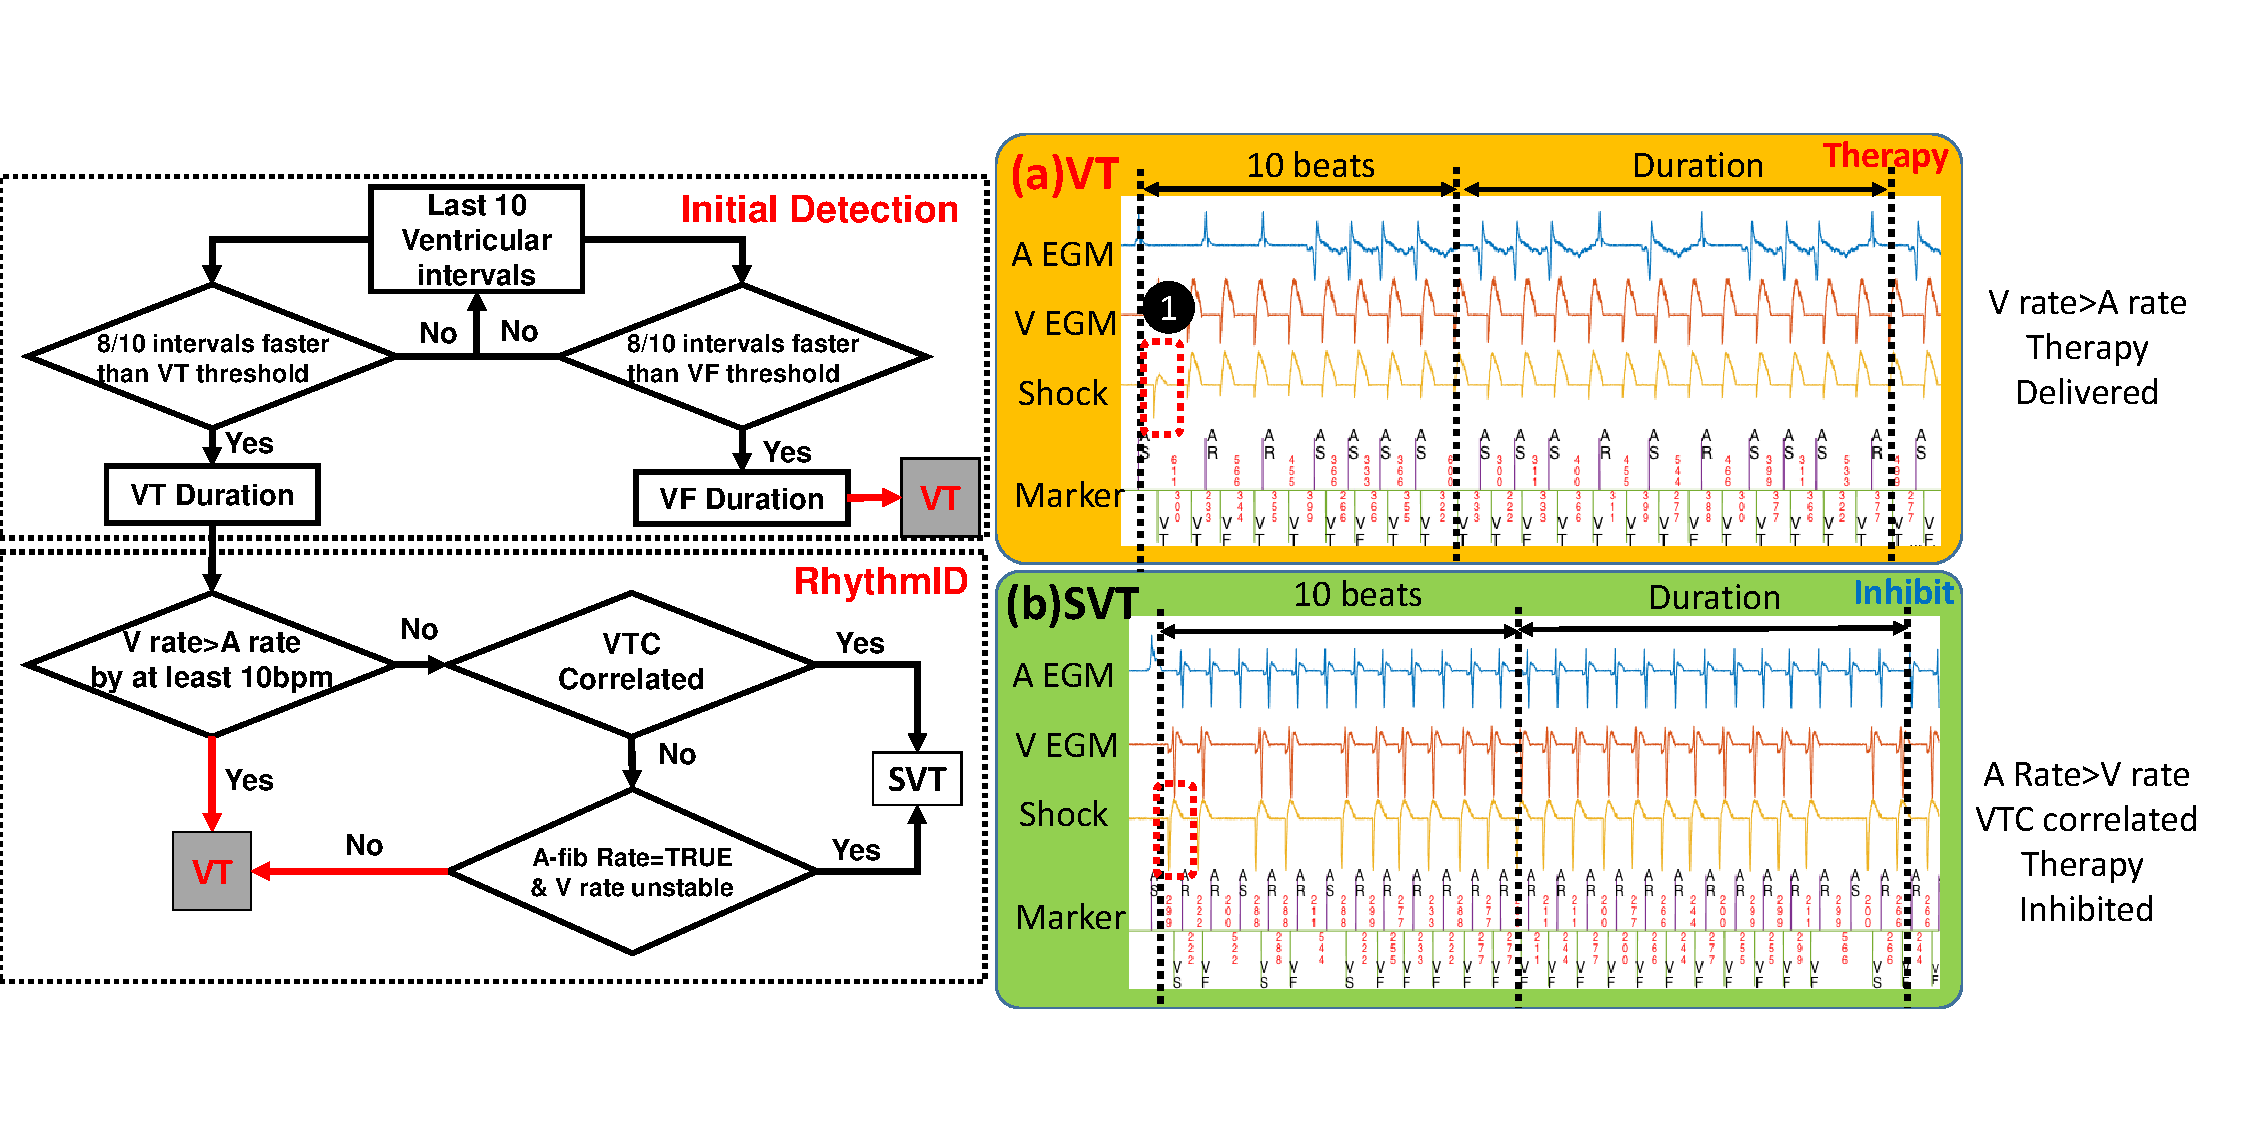
\includegraphics[scale=0.38]{figs/BS_det.pdf}
	\vspace{-10pt}
	\caption{\small SVT/VT detection algorithm by Boston Scientific \cite{compass}. The two cases on the right illustrate two different decisions by the algorithm. (a) illustrates a sustained VT case where at the end of the Duration, the ventricular rate is faster than the atrial rate. The algorithm correctly identified the rhythm as VT and delivered therapy. (b) illustrates a SVT case where at the end of the Duration, the ventricular rate is slower than the atrial rate. Then by comparing the EGM morphology in the Shock channel (Marker 1) with the stored NSR template (Marker 2) for the last 10 EGM events, the algorithm decided that the morphology is correlated, therefore therapy is inhibited.}
	\label{fig:BS_det}
\end{figure*}

\subsubsection{Rhythm ID}
Rhythm ID's decision tree is shown in Fig.~\ref{fig:BS_det}.
Rhythm ID detects an episode by continuously examining the last 10 ventricular intervals and comparing them with VT and VF thresholds. 
If 8/10 intervals are shorter than the VF threshold for a certain pre-set \emph{VF Duration} (e.g., 2.5 seconds) then the algorithm declares VF.
Otherwise, if 8/10 intervals are shorter than the VT threshold for a certain VT Duration, then further discriminators are used.
First, if the ventricular rate is greater than the atrial rate for the last 10 ventricular beats, Rhythm ID will determine the condition is VT.
Otherwise, the Vector Timing and Correlation (VTC) discriminator~\cite{VTC} compares EGM morphology of the last 10 ventricular events with an EGM \emph{template} saved during NSR.
VTC is based on the assumption that the EGM morphology of the shock channel during VT is different from its morphology during SVT and NSR.
If the correlation between the current EGM's morphology and the stored NSR morphology is above a pre-set threshold, the current rhythm is more likely to be SVT than VT, and therapy is withheld.
Otherwise, if the atrial rate is equal to a pre-set fibrillation rate and the variance of the ventricular interval length exceeds a certain limit, the algorithm decides it's an SVT. 
Otherwise, it decides this is a VT.
%As shown in Fig. \ref{fig:BS_det}(b), at the end of the duration, the atrial rate is faster than the ventricular rate. 
%The morphology in the shock channel is similar to the NSR morphology (red dashed) so VTC is correlated and therapy is inhibited.
%As a comparison the morphology during VT is different from the NSR morphology (Marker 1 in Fig. \ref{fig:BS_det}).

\subsubsection{PR Logic+Wavelet}
PRL+W also utilizes rate-based and morphology-based discriminators similar (but not identical) to Rhythm ID.
The morphology discriminator used in PRL+W  is similar to VTC in Rhythm ID, but operates in the wavelet domain~\cite{Wavelet}.
PRL+W also continuously compares the pattern of atrial and ventricular activation to 19 pre-defined patterns~\cite{Singer}.
Each pattern is associated to a heart condition, like Sinus Tachycardia or VT.
A match between the current activity and one of the pre-defined patterns is used as an indication that the current rhythm is explained by the associated condition.

\subsection{Validation}
\label{sec:validation}
%\begin{figure}[t]
%	\centering
%	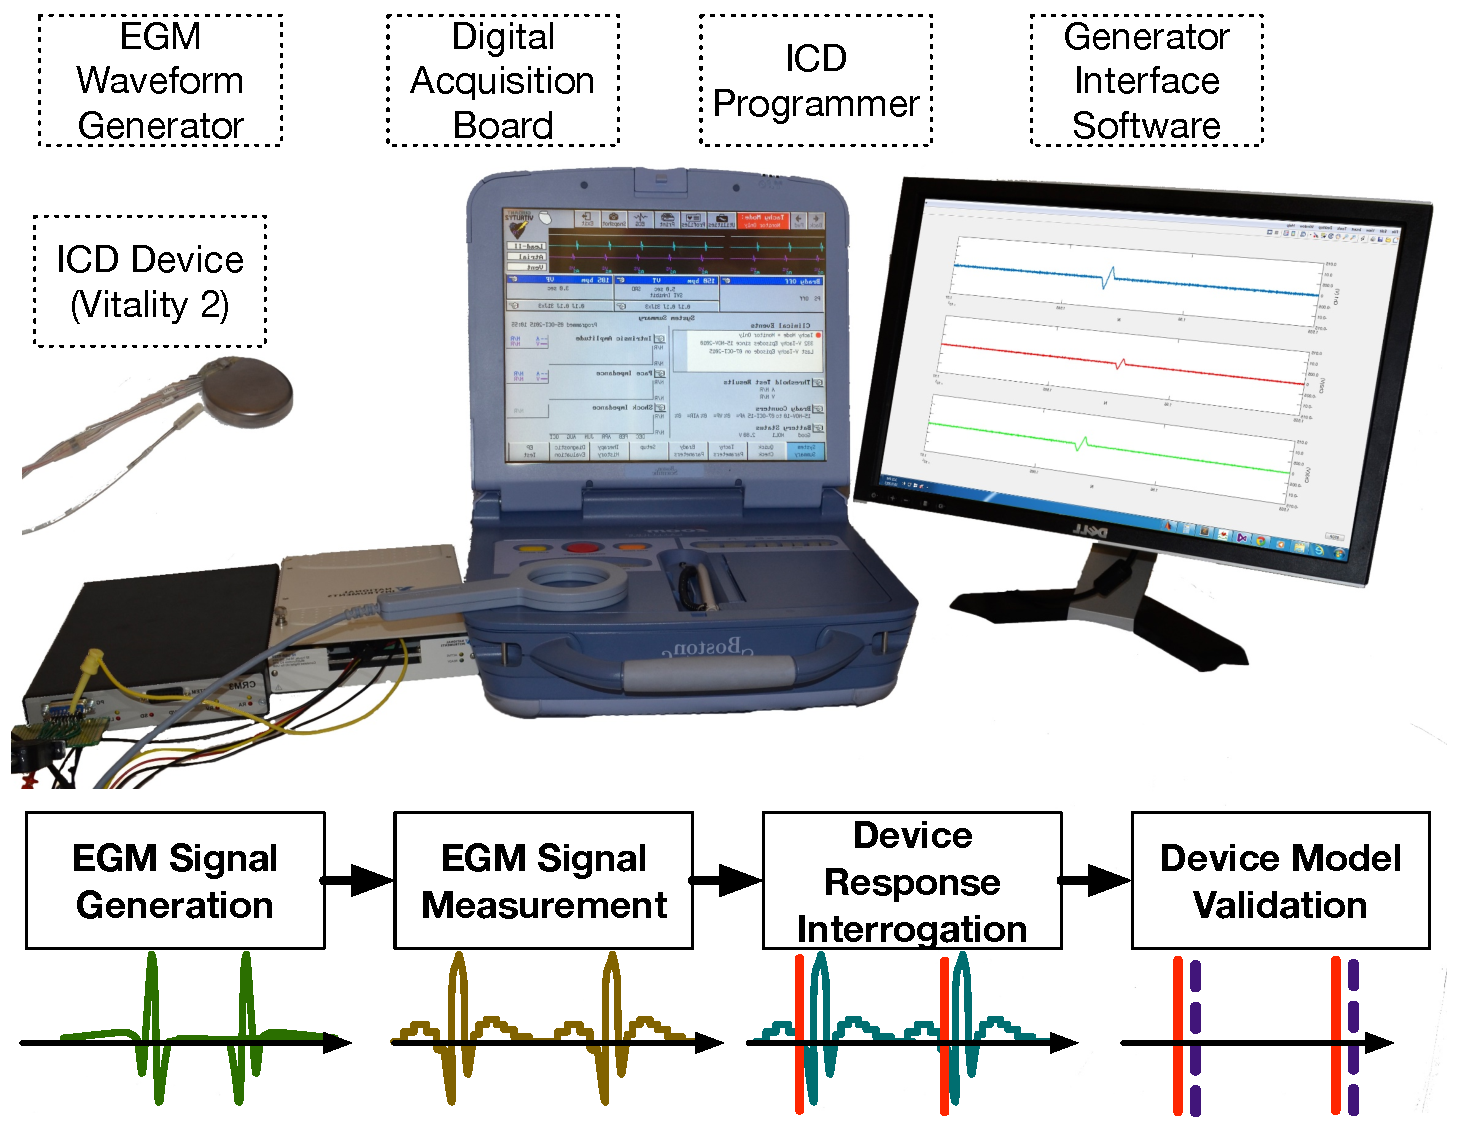
\includegraphics[scale=0.28]{figures/figValidationSetup.pdf}
%	\vspace{-10pt}
%	\caption{\small Model Validation. 14 different scenarios were generated from the EGM waveform generator for Boston Scientific and input into the Vitality 2 ICD. The input signal was acquired through the DAQ board and applied to the device model implementation. The ICD response was interrogated using the ICD programmer and compared to the output of the device model.}
%	\vspace{-10pt}
%	\label{fig:validationSetup}
%\end{figure}

\begin{figure}[t ]
	\centering
	\includegraphics[scale=0.28]{figures/figScreenshot.pdf}
	\caption{\small Example of validation output screenshots (Ventricular fibrillation) showing matching therapy decision for the ICD and our implementation.}
	\vspace{-10pt}
	\label{fig:validation}
\end{figure}

Conformance testing was used to validate the software implementations of the Vitality II device by Boston Scientific. 
The validation hardware setup is illustrated in Fig.~\ref{fig:validation}. 
14 different scenarios were specified and programmed into an EGM Waveform generator (CRM3 Simulator, Guidant, USA) such that it would output a signal to the connected Vitality II device.
The various scenarios traverse 7 out of 9 branches of the detection algorithm for Boston Scientific described in Sec. \ref{sec:svtvt} and shown in Fig. \ref{fig:BS_det}. 
The response of the ICD interrogated using an ICD programmer (ZOOM Latitiude, Boston Scientific).
As the waveform was applied to the ICD, the waveform was simultaneously acquired using a National Instruments DAQ board.
The recorded waveform was then applied to the device model and response was compared.
Fig. \ref{fig:validation} shows an example of one such scenario, specificallly VF. 
In this case, the software model matched to the decision of the actual ICD which also determined that therapy should be applied.

In all scenarios, the decision of model conformed to that of the ICD. 
The remaining two branches were not reachable due to the limited output capability of the programmer.
The Medtronic software implementation can be validated using a similar process.

\section{Results}

\subsection{The rate of inappropriate therapy}
\label{sec:rate inapp}
%\todo[inline]{justify episode-level rates and not patient-level}
The first objective of the MBCT is to estimate the rate of inappropriate detection $\bar{t}$ for each of the two algorithms for all arrhythmias combined, i.e., for the entire synthetic cohort.
The rate of inappropriate therapy is defined as
\[\bar{t} = \frac{\text{Number of inappropriately applied therapies}}{\text{Number of applied therapies}}\]
From this we can confirm or invalidate the assumption that Rhythm ID outperforms PRL+W.
We generated a synthetic cohort of 11,400 heart instances, equally distributed among the 19 arrhythmias.
The number of instances was obtained from a Monte Carlo calculation.% whose details follow the presentation of the results.

\textbf{Conclusion 1: PRL+W delivers less inappropriate therapy.}
The obtained rates of inappropriate detection were 6.65\% for Boston Scientific and 2.91\% for Medtronic (P < 0.0001), assuming an equal number of patients from each arrhythmia in the synthetic cohort.
The corresponding relative improvement \emph{of Medtronic over Boston Scientific} is 56\%.
In other words, the MBCT reveals that the PRL+W algorithm from Medtronic actually differentiates between VT and SVT better than Rhythm ID from Boston Scientific.
Our findings are consistent with the observations of the RIGHT trial itself~\cite{GoldABBTB11_RIGHTresults}.

\textbf{Conclusion 2: result holds across population characteristics.}
The above rates were obtained under the assumption that each arrhythmia is equally represented in the cohort.
A significant feature of MBCT is that it allows us to study the endpoint of interest (here, rate of inappropriate detection) on a variety of populations, which have the various arrhythmias in different proportions.
This may not be feasible in a real clinical trial, which has to contend with the population present at the clinical centers where the trial is conducted.
We may then ask: does PRL+W maintain a lower rate of inappropriate detection across different populations?
To answer this question, we varied the distribution of the arrhythmias in the synthetic cohort, and re-computed the cohort-wide rates of inappropriate therapy.
Fig. \ref{fig:popvar8} shows the results for 10 random variations of the arrhythmia distribution.
It can be seen that indeed, PRL+W maintains a better rate of arrhythmia discrimination (and by inference, less inappropriate therapy) across the board.
%Thus the results are robust to the characteristics of the population under study.
%\mynote{SD}{Delete last sentence}

\begin{figure*}[t]
	\vspace{-10pt}
\centering
\vspace{-10pt}
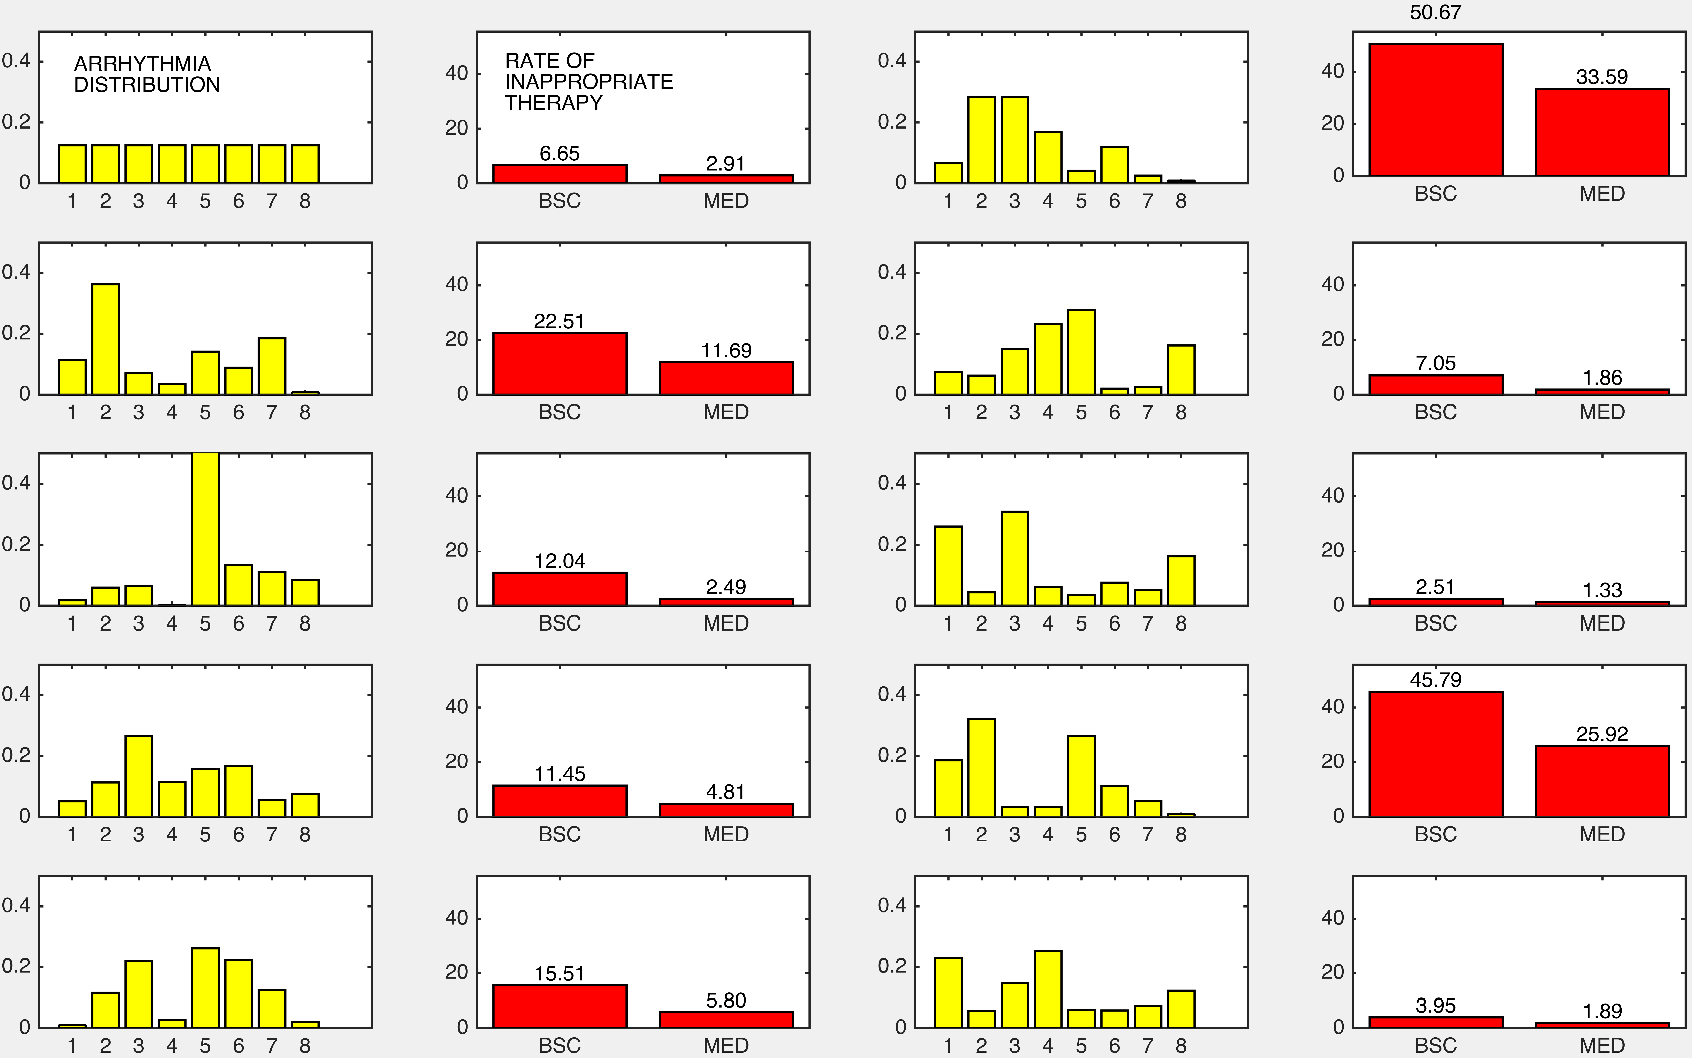
\includegraphics[scale=0.4]{figures/popvar9}
\caption{\small Rate of inappropriate detection ($2^{nd}$ and $4^{th}$ columns) for different arrhythmia distributions ($1^{st}$ and $3^d$ columns). The arrhythmias are (left to right on the x axis): Atrial fibrillation, Atrial flutter, Premature Ventricular Complexes, Nonsustained Ventricular Fibrillation, Supraventricular Tachycardia, Sinus Brady-Tachy, Ventricular Fibrillation, Ventricular Tachycardia \cite{josephson}. The top left distribution is uniform, and the bottom right distribution is that of the baseline characterization in RIGHT \cite{GoldABBTB11_RIGHTresults}.}
\label{fig:popvar8}
\end{figure*}

This illustrates very well the benefit that an MBCT can bring to the planning of an RCT: the fact that Rhythm ID could not be shown to be better than PRL+W %(let alone 25\% better as was hypothesized by the investigators) 
can cause the investigators to re-consider their assumptions and the feasibility of the trial.
In this case, the MBCT casts doubt on the assumed \emph{direction} of the effect, i.e. whether intervention is better than control, or the other way around.
This early check can mean the difference between an expensive trial that fails at showing the desired effect, and a trial that is appropriately sized to demonstrate the desired effect size.

%While we will not know the true distribution of the arrhythmias in the \ac{RCT} until its completion, 
Thus, while an MBCT does not replace or mimic the RCT since we can not capture patient-level outcomes of the therapy, it can provide  but \emph{early insight} at a small fraction of the RCT cost and duration and without the ethical issues.	 

%\textbf{Sample size calculation for MBCT}.
%The rate is naturally computed as the mean of a random variable.
%Namely, it is the mean of the variable $t$ which equals 1 if the episode is a VT/VF for which therapy was applied, and 0 if it's a VT/VF for which therapy was withheld.
%To get reliable estimates for this rate, we use a standard Monte-Carlo calculation under the assumption that the estimate of the mean is normally distributed around the true mean. 
%This is justified by the central limit theorem and the fact that we can generate a very large number of hearts for each rhythm.
%By choosing a confidence interval width of 0.001 around the mean, we obtain a sample size of 9,604 hearts.
%In our experiments we used 11,400 to decrease the empirical variance of the estimate.
%The 95\% confidence interval around the mean estimate is given by $CI = \hat{t} \pm z_{95}\frac{S_t}{\sqrt{n}}$, 
%where $\hat{t}$ is the mean estimate, $z_c$ is the $c\%$ confidence level (so $z_{95}=1.96$), 
%$S_t$ is the empirical variance, 
%and $n$ is the number of Monte Carlo simulations, i.e., the number of heart instances we will generate and simulate for a given rhythm.
%The larger the number of simulations $n$, the tighter the confidence interval around the estimate.
%The rates we estimate fall in the range $[0,1]$ and are significant to the second decimal digit.
%Because we are considering all arrhythmias combined, we assume a conservative empirical variance $S_x$ to be 0.05, (validated experimentally) and set the desired confidence interval half-width to 0.001:
%\[\1.96\frac{0.05}{\sqrt{n}} = 0.001\]
%This yields $n = 9604$.
%In the experiments we use $n=11400$ to help guarantee the assumed empirical variance.
%The obtained empirical variance is invariably much smaller than 0.05.

%The obtained results for sensitivity and inappropriate therapy rate are shown 
%\begin{table}[b]
%	\smallcaption{Sensitivity and inappropriate therapy rate.}
%	\begin{tabular}{|p{1.9cm}|c|p{2.5cm}|}
%		\hline             & \textbf{Boston Sci.}(\%)   & \textbf{Medtronic} (\%)\\
%		\hline Sensitivity &  100                   &  100  \\ 
%		\hline Inappropriate therapy rate &  6.65                   &  2.91 \\ 
%		\hline 
%	\end{tabular}
%	\label{table:total nbs}
%\end{table} 

%We may also define a hypothesis test, which we illustrate for the rate of inappropriate therapy.
%The null hypothesis $H_{0,t}$ is that the rates for $\bar{t}$ are equal for Medtronic and Boston Scientific devices.
%\[H_{0,t}: \bar{t}_{MED} = \bar{t}_{BSC}  \]
%The alternative hypotheses are that the rates are not equal.
%In all that follows, `effect size' refers to the relative difference between the two rates.
%
%We assume an effect size of 27\%: this is based on the \emph{episode-level} inappropriate therapy rates reported in RIGHT (Table 2 of \cite{GoldABBTB11_RIGHTresults}).
%(Note that some of those reported results, however, were not statistically significant at the 5\% significance level).
%At the 5\% significance level and 90\% power, this yields a sample size of 11160.
%% with an assumed BSC rate of 0.08.
%We used 11400 instances in our MBCT.
%The results were inappropriate therapy rates $\bar{t}_{BSC}= 0.0291$ and $\bar{t}_{MED} = 0.0665$, with an effect size (relative to Medtronic's algorithm) of 56\% with $P << 10^{-3}$.
%Thus the null hypothesis of equality of inappropriate therapy rates can be rejected.

\subsection{Condition-level rates}
\label{sec:condition-level}
Having a heart model allows us to better estimate the \emph{sensitivity} and \emph{specificity} of the diagnostic algorithms' performance, something which is not possible in a clinical trial because the device only records a limited number of episodes.
These are defined as
\[ \text{Sensitivity} = \frac{\text{Number of correctly classified VTs}}{\text{Number of true VTs}}\]
\[ \text{Specificity} = \frac{\text{Number of correctly classified SVTs}}{\text{Number of true SVTs}}\]
In words, the sensitivity measures how well the device recognizes VTs.
Specificity measures how well the device discriminates between VT and SVT.
An ideal device would have 100\% sensitivity and specificity.
Unfortunately, these are typically competing goals: the more sensitive the device, the more likely it will mis-diagnose some SVTs as VTs, so its specificity will drop.
%During a clinical trial, the implanted ICD is typically set to record only treated episodes, so it is not possible to obtain all episodes and measure specificity.
%Moreover, if a VT episode is non-sustained, it won't receive therapy and won't be recorded, so it's not possible to measure sensitivity.
%Even if the device were set to record all episodes whether treated or not, memory limitations mean that it won't record everything.

We calculated sensitivity and specificity in our MBCT, and report them in Table \ref{table:vtsvt} on a per-arrhythmia basis.
The conditions are drawn from RIGHT's baseline characterization \cite{GoldABBTB11_RIGHTresults}.
Specificity is reported for SVTs and sensitivity is reported for VTs.
It can be seen from these results that in our synthetic cohort, Atrial flutter and other Supraventricular tachycardias are the main source of inappropriate detection for Rhythm ID compared to PRL+W.
In the case of Atrial flutter, Rhythm ID categorizes it inappropriately as VT for 41.7\% of the cases.

Condition-level analysis pinpoints the specific pathways of the discrimination algorithm which must be addressed to reduce the device's rate of inappropriate therapy. It is difficult to get such insight through an RCT as the patient population is fixed and the conditions are determined retroactively. Such analysis can be further used to investigate condition distributions across different patient population types (e.g. abnormal heart rhythms in children vs geographic region-specific or race-specific condition distributions).   

\begin{table}[t]
	\vspace{-10pt}
	Specificity and sensitivity.
\begin{tabular}{|p{2.8cm}|p{1.5cm}|p{1.5cm}|c|}
	\hline Arrhythmia & Rhythm ID & PR Logic + Wavelet  & P value \\ 
	\hline &	\multicolumn{2}{|c|}{\textbf{Specificity} (\%)}& \\
	\hline Atrial Fibrillation & 99.8 & 99.6 & 0.3167 \\ 
	\hline \cellcolor{blue!25} Atrial flutter & 58.3 & 79.33 & <0.0001 \\ 
	\hline Premature ventricular complexes & 100 & 100 & 1 \\ 
	\hline Nonsustained ventricular tachycardia & 100 & 99.8 & 0.3171 \\ 
	\hline \cellcolor{blue!25} Other Supraventricular tachycardia & 96.3 & 99.7 & <0.0001 \\ 
	\hline Brady-Tachy & 100 & 98.83 & 0.0079 \\ 
		\hline
	\hline &	\multicolumn{2}{|c|}{\textbf{Sensitivity} (\%)} & \textbf{P value}\\
	\hline Ventricular fibrillation & 100 & 100 & 1 \\ 
	\hline Ventricular tachycardia & 100 & 100 & 1 \\ 
	\hline 
\end{tabular} 
\vspace{-10pt}
\label{table:vtsvt}
\end{table}

 \subsection{Effect of Device Parameters on Discriminating Capability}
ICDs have a number of parameters which can be tuned to accommodate specific patient conditions by the physicians. 
%For example, pacemakers have over 400 possible settings for which the physician may tune less than 5 parameters during implantation and in follow-up visits, while leaving the other settings at their default values.
Currently there are very few clinical results on the effect of tuning parameters and their effect on sensitivity and specificity~\cite{maditrit}.
One of the main causes of VT/SVT mis-classifications is inappropriate parameter settings~\cite{wrong_sensing}.
In order for the physicians to set appropriate parameters, it is very important to understand how the change of one parameter can affect the discriminating capability of the device.
It is costly to experiment this on real patients.
With MBCT, one can use the same population across multiple devices with different parameter settings at virtually no cost. 
%The resulting trends can provide valuable insights to physicians.

In this section, we use MBCT to demonstrate the effects of changing two common parameters on SVT/VT discrimination specificity.
The first parameter is the \emph{\textbf{duration}} of arrhythmia before the ICD makes a therapy decision. 
For Boston Scientific ICD the value can be set to 1 to 30 seconds.
In this experiment we explore the values \{1,2,3,4,5,8,10\}.
The equivalent parameter for Medtronic ICD is the number of consecutive fast ventricular intervals which can be set from 8 to 20 beats.
In this experiment we explore the values \{8,10,12,16,18,24,30\} which roughly correspond to the parameters of Boston Scientific ICD.
Intuitively, with a longer duration the device can examine a longer history of the arrhythmia episode, and also allows a greater chance for the arrhythmia to self-terminate. 
This can prevent inappropriate therapy.
Setting the duration too long can also delay and in some cases withhold appropriate therapy. 
These results are in agreement with the recently conducted ADVANCE-III RCT which showed that longer arrhythmia detection windows reduce shocks for Medtronic ICDs~\cite{advance3}.

The second parameter we varied is the \emph{\textbf{VF threshold}}.
For both devices, if the ventricular rate is faster than the VF threshold for a period of time the devices will deliver therapy without going into the SVT/VT discrimination algorithm. So a higher VF threshold means that more signals are passing through the discrimination algorithm.
In this experiment we explored the values \{170,184,200\} for both algorithms.
Intuitively the higher the threshold, the more episodes will be examined by the SVT/VT discrimination algorithm, which may increase specificity.
%However, VTs with rate less than the threshold may also be classified as SVT, causing missed therapies.\\
\newline\textbf{Conducting the Model-based Clinical Trial}. 
For each of the 21 parameter combinations described above, we ran a MBCT with 11,400 EGM episodes on both device models. 
%Each MBCT took approximately 3 hours on a 3GHz Intel Xeon processor with 8 cores. The resulting specificity values are shown in Fig. \ref{fig:parameter}. 
From the results we observe that for both algorithms the specificity increases monotonically with the length of the duration.
When the duration is longer than 5, sensitivities dropped below 100\%, which is in line with the intuition.
\begin{figure}[t]
	
		\centering
		\vspace{-10pt}
		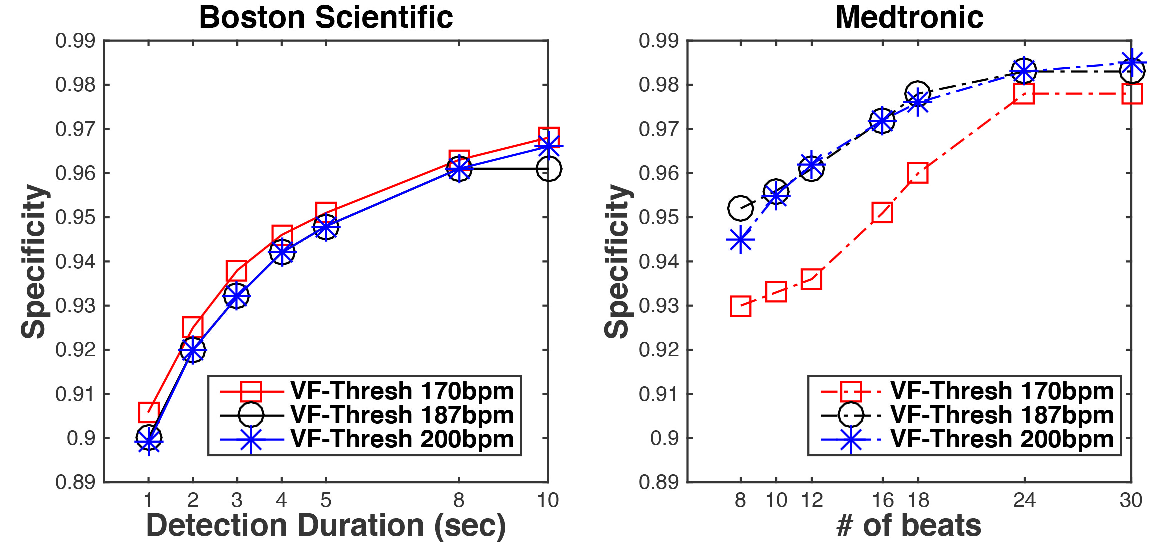
\includegraphics[width=0.45\textwidth]{figs/parameter.pdf}
		\caption{\small Effects of Duration and VF threshold parameters on Specificity}
		\vspace{-10pt}
		\label{fig:parameter}
\end{figure}
However, Rhythm ID and PRL+W displayed opposite trends for the VF threshold.
%This agrees with the RIGHT finding that the rate of inappropriate therapy is highest for \acp{VT} with a rate $\leq 175$bpm \cite{GoldABBTB11_RIGHTresults}.
For PRL+W, the specificity increased when the VF threshold was increased from 170BPM to 184BPM - i.e. a higher threshold admits more signals through the discrimination algorithm which performs better across all rates.
For Rhythm ID the specificity dropped when the VF threshold was increased from 170BPM to 184BPM - i.e. the discrimination algorithm is less effective at higher rates. 
One possible interpretation of the result is that the Boston Scientific algorithm is more prone to inappropriate therapies for SVTs with ventricular rate between 170BPM to 184BPM, which may be a useful for the physicians to consider during parameter settings. 



\section{Discussion}
\label{sec:discussion}

The above experiment has illustrated a practical application of the MBCT approach in the use of computer modeling for the support of clinical trial planning and execution.
We now present the medically relevant limitations of this particular experiment, then discuss the MBCT approach in general.
First, we did not account for post-shock detection (a phase of detection that follows the delivery of therapy), which was part of the RIGHT results.
The Onset discriminator was not implemented so the results exclude its effects.
RIGHT included both dual-chamber and single-chamber devices, whereas we only implemented the algorithms for dual-chamber devices.
For the VTC and Wavelet algorithms, the literature did not specify which samples are taken from the electrogram. 
We chose to sample the electrogram uniformly in time, and validated that this gives correct results.
%In the clinical setting, some of the programmable parameters of the device are set by the physician based on the current state of the patient. 
%It is not currently possible to model this process.
%However, it does point the way to an interesting application of MBCT, namely studying the sensitivity of a trial's results to parameter setting strategy.

Clinical trials study the effect of an intervention \emph{in the patient}, and report patient-level results (e.g., ``The event of interest was observed in X\% of patients in Group 1''). 
Our results are at the condition level: they take the form ``the event of interest was observed in X\% of generated conditions".
To produce patient-level estimates requires an estimate of how conditions are distributed among patients. 
This low-level data is not readily available.

It is important to stress that in general, one should not expect \emph{absolute numbers} from an MBCT to match those from a clinical trial, nor should this be the goal of the MBCT.
For example, in this work, it is unlikely that our MBCT will yield rates of inappropriate therapy that are equal to the rates obtained by RIGHT itself.
The reasons for this are many:
\begin{itemize}
	\item Many factors that affect the outcomes of the trial (such as changes in patient lifestyle) are not modeled.
	\item The adjudication of episodes in RIGHT (and other trials) is limited by the fact that only therapy episodes were recorded by the devices.
	The adjudication process is further limited by the lack of surface EKGs, which makes it hard to reliably distinguish certain atrial arrhythmias. 
	Neither of these is a limitation in MBCT since we have the ground truth: we know exactly what arrhythmia is being simulated by the model.  Furthermore, the AAEL signals have both device electrograms (EGMs) and the corresponding surface EKGs which allow for precise adjudication.  
	\item Experts may disagree on how to adjudicate the more complex episodes, so our classification of episodes from the AAEL database and the classification of the RIGHT investigators have an irreducible discrepancy.
	Again, this will affect the statistics that they and we compute.
\end{itemize}

That said, we can expect that a good heart model will reveal \emph{the trend} of the results, such as improvement of intervention over control or not, as shown in this paper. 
